\section{Analysis of \sse Output}\label{sec:ana}

Each execution of \sse creates a folder for analysis output.
Apart from the general log files, where all plugins write important messages, some plugins also create separate files.
One file for memory ..., one with LLVM bytecode, one ...\todo{..}

The most important information about \sse's general execution is accumulated in \textit{messages.txt}.
Backbone of this file is information about all execution paths, at which memory addresses they were forked, how they are constrained, when and why they were terminated, and much more.
%But it is also used by other plugins...

Thanks to the clear structure of \textit{messages.txt}, it can be used as input for a custom Python script. This script was written in order to visualise the tree of execution paths graphically, which serves as a great help with understanding path forking behaviour.
Figure \ref{} shows the root\todo{?} of the tree of execution paths of \app.
Each box represents an execution state, lines pointing to another state symbolise a fork of the execution state.
The hex number at the origin of each edge is the memory address in which the state was forked.
Edges are labelled with all constraints that need to be respected in the corresponding execution state.
Blue state boxes indicate one connection to the internet so far, yellow two and red three.
The text below each leaf shows the output of the \textit{TestCaseGenerator} plugin for this execution path.

It is only the root because....

The whole graph (without constraints) looks as folllows:...

\begin{figure}
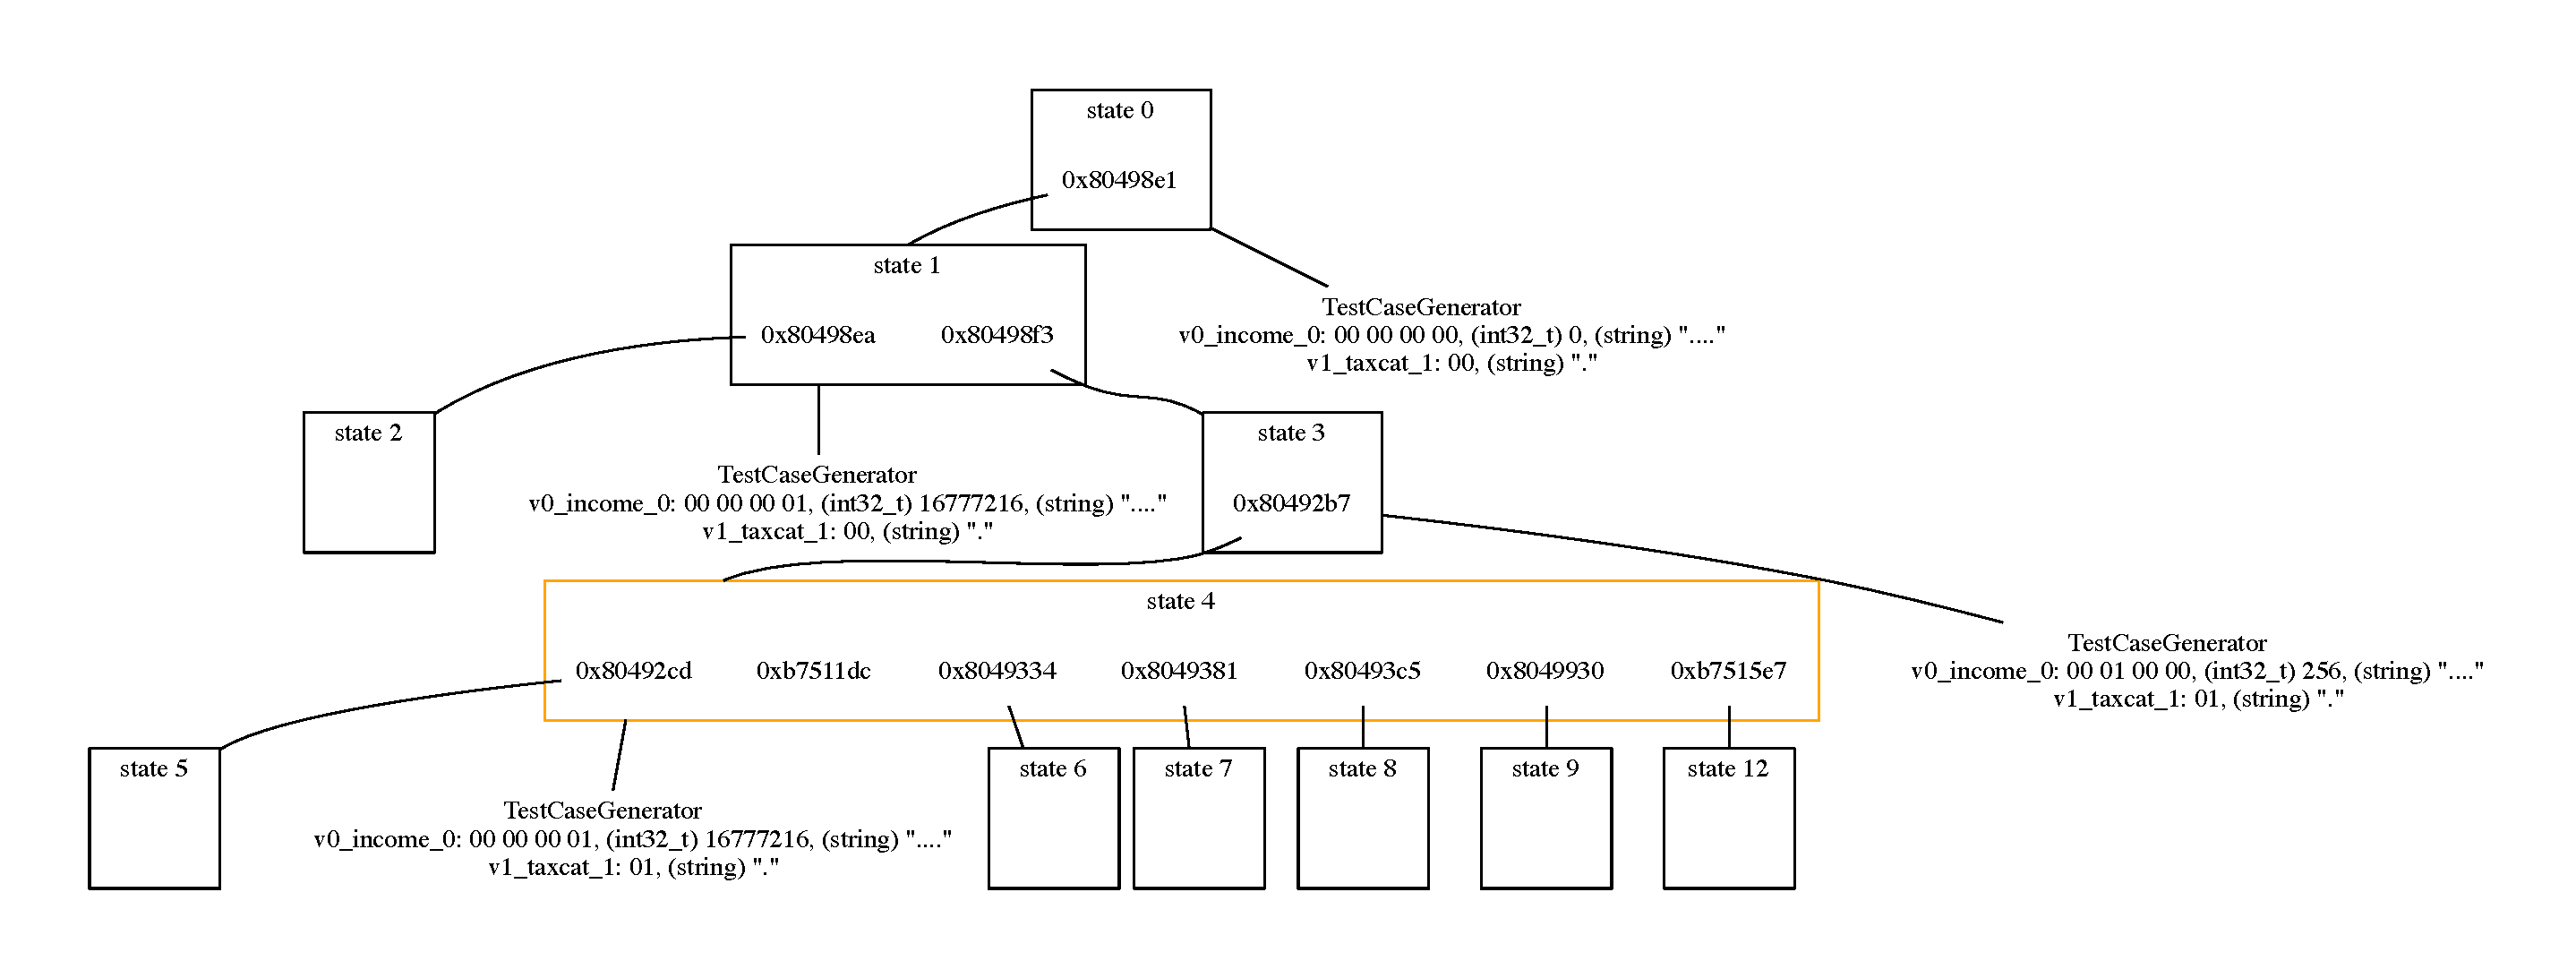
\includegraphics[width=\columnwidth]{small}
\caption{Graph}
\label{fig:tree}
\end{figure}



\iffalse
§6	Interpretation of S2E analysis output
		> Execution Traces
		> Gefundene Privacy-Probleme
		> Eventuell nicht gefundene Sachen
		> Probleme bei der Analyse
\fi